% !TEX program = lualatex
% Knowledge Graph + JEPA World Models for Magic: The Gathering
% From Game Engine to Structured Imagination
%
% Compile: lualatex kg_jepa_world_model.tex  (twice for references)
% Or:      pdflatex kg_jepa_world_model.tex

\documentclass[aspectratio=169, 11pt]{beamer}

% -- Theme ----------------------------------------------------------
\usetheme{Madrid}
\usecolortheme{seahorse}
\setbeamertemplate{navigation symbols}{}
\setbeamertemplate{footline}[frame number]
\setbeamertemplate{itemize items}[circle]

% -- Packages -------------------------------------------------------
\usepackage{tikz}
\usetikzlibrary{
  positioning, arrows.meta, shapes.geometric, fit, calc,
  backgrounds, decorations.pathreplacing, matrix
}
\usepackage{booktabs}
\usepackage{amsmath, amssymb}
\usepackage[utf8]{inputenc}
\usepackage{listings}
\usepackage{xcolor}
\usepackage{textcomp}

% -- Colors ---------------------------------------------------------
\definecolor{mtgblue}{HTML}{1E3A5F}
\definecolor{mtgred}{HTML}{C13A28}
\definecolor{mtggreen}{HTML}{2D6A2E}
\definecolor{mtggold}{HTML}{D4A843}
\definecolor{kgpurple}{HTML}{6B3FA0}
\definecolor{jepaorange}{HTML}{E07020}
\definecolor{codebg}{HTML}{F5F5F0}
\definecolor{lightgray}{HTML}{E8E8E8}

% -- Listings -------------------------------------------------------
\lstset{
  basicstyle=\ttfamily\scriptsize,
  backgroundcolor=\color{codebg},
  frame=single,
  rulecolor=\color{lightgray},
  breaklines=true,
  columns=fullflexible,
  keywordstyle=\color{mtgblue}\bfseries,
  commentstyle=\color{mtggreen},
  stringstyle=\color{mtgred},
}

% -- Metadata -------------------------------------------------------
\title[KG + JEPA World Models for MTG]{%
  Knowledge Graph + JEPA World Models\\
  for Magic: The Gathering}
\subtitle{From Game Engine to Structured Imagination}
\author{opposition-agents-playing-mtg}
\date{March 2026}

% ===================================================================
\begin{document}

% -- Title ----------------------------------------------------------
\begin{frame}
  \titlepage
\end{frame}

% -- Outline --------------------------------------------------------
\begin{frame}{Outline}
  \tableofcontents
\end{frame}


% ===================================================================
\section{Part I --- The Project}
% ===================================================================

% -- Slide 1 --------------------------------------------------------
\begin{frame}{The Problem Statement}
  \begin{center}
    \large\bfseries Magic: The Gathering is the hardest popular game for AI.
  \end{center}
  \vspace{0.3cm}
  \begin{table}
    \centering\footnotesize
    \begin{tabular}{@{}lcccc@{}}
      \toprule
      \textbf{Dimension} & \textbf{Chess} & \textbf{Go} & \textbf{Poker} & \textbf{MTG} \\
      \midrule
      State space         & $\sim10^{47}$  & $\sim10^{170}$ & $\sim10^{6}$    & $\mathbf{\sim10^{800+}}$ \\
      Unique pieces/cards & 6              & 1               & 52              & \textbf{28,000+} \\
      Hidden information  & None           & None            & 2 cards         & \textbf{50--90 cards} \\
      Action space (avg)  & $\sim$30       & $\sim$250       & $\sim$5         & \textbf{0--100+} \\
      Multi-modal outcomes& Determ.        & Determ.         & Draw-dep.       & \textbf{Stack + triggers} \\
      Rule complexity     & $\sim$50 pp    & $\sim$20 pp     & $\sim$5 pp      & \textbf{$\sim$260 pp} \\
      \bottomrule
    \end{tabular}
  \end{table}
  \vspace{0.3cm}
  \begin{itemize}
    \item Chess fell to tree search. Go fell to neural MCTS. Poker fell to CFR.
    \item \textbf{MTG hasn't fallen to anything.}
  \end{itemize}
\end{frame}

% -- Slide 2 --------------------------------------------------------
\begin{frame}{Why MTG Matters Beyond Games}
  MTG is a microcosm of real-world decision problems:
  \vspace{0.3cm}
  \begin{columns}[T]
    \begin{column}{0.48\textwidth}
      \footnotesize
      \begin{tabular}{@{}ll@{}}
        Hidden information         & Military, business \\
        Partial observability      & Medicine, finance \\
        Combinatorial explosion    & Drug discovery \\
        Long-horizon planning      & Supply chain \\
      \end{tabular}
    \end{column}
    \begin{column}{0.48\textwidth}
      \footnotesize
      \begin{tabular}{@{}ll@{}}
        Adversarial opponents    & Cybersecurity \\
        Rule-governed interaction & Legal reasoning \\
        New cards every 3 months  & Evolving envs \\
      \end{tabular}
    \end{column}
  \end{columns}
  \vspace{0.5cm}
  Solving MTG advances state-of-the-art in:
  \begin{itemize}
    \item Planning under uncertainty in large POMDPs
    \item Zero-shot generalization to new rules and entities
    \item Opponent modeling with hidden state inference
    \item Structured reasoning over complex rule systems
  \end{itemize}
  \vspace{0.3cm}
  \begin{center}
    \textit{If you can build an agent that plays MTG well,\\
    you've solved a lot of hard AI in one go.}
  \end{center}
\end{frame}

% -- Slide 3 --------------------------------------------------------
\begin{frame}{This Repository: opposition-agents-playing-mtg}
  A complete research framework --- not a toy prototype.
  \vspace{0.3cm}
  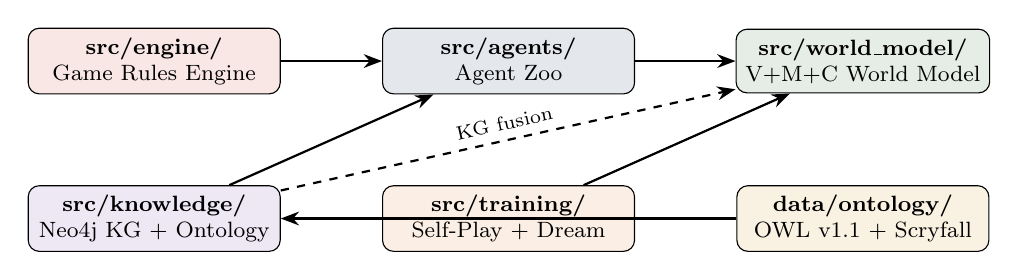
\begin{tikzpicture}[
      every node/.style={font=\footnotesize},
      pkg/.style={draw, rounded corners, fill=mtgblue!10, minimum width=3.2cm, minimum height=0.7cm, align=center},
      label/.style={font=\scriptsize\ttfamily, text=mtgblue},
    ]
    % Packages
    \node[pkg, fill=mtgred!12] (engine) at (0, 0) {\textbf{src/engine/}\\Game Rules Engine};
    \node[pkg, fill=mtgblue!12] (agents) at (4.5, 0) {\textbf{src/agents/}\\Agent Zoo};
    \node[pkg, fill=mtggreen!12] (wm) at (9, 0) {\textbf{src/world\_model/}\\V+M+C World Model};
    \node[pkg, fill=kgpurple!12] (kg) at (0, -2) {\textbf{src/knowledge/}\\Neo4j KG + Ontology};
    \node[pkg, fill=jepaorange!12] (train) at (4.5, -2) {\textbf{src/training/}\\Self-Play + Dream};
    \node[pkg, fill=mtggold!15] (data) at (9, -2) {\textbf{data/ontology/}\\OWL v1.1 + Scryfall};

    % Arrows
    \draw[-{Stealth}, thick] (engine) -- (agents);
    \draw[-{Stealth}, thick] (agents) -- (wm);
    \draw[-{Stealth}, thick] (kg) -- (agents);
    \draw[-{Stealth}, thick] (train) -- (wm);
    \draw[-{Stealth}, thick] (data) -- (kg);
    \draw[-{Stealth}, thick, dashed] (kg) -- (wm) node[midway, above, sloped, font=\scriptsize] {KG fusion};
  \end{tikzpicture}
  \vspace{0.2cm}
  \begin{columns}[T]
    \begin{column}{0.32\textwidth}
      \scriptsize
      \textbf{Engine}: Zones, stack, priority, combat, triggers, layers, SBAs
    \end{column}
    \begin{column}{0.32\textwidth}
      \scriptsize
      \textbf{Agents}: Random, LLM, WorldModel, ActiveInf, Combo, Opponent
    \end{column}
    \begin{column}{0.32\textwidth}
      \scriptsize
      \textbf{New}: KGEncoder, JEPA predictor, dual-input training
    \end{column}
  \end{columns}
\end{frame}

% -- Slide 4 --------------------------------------------------------
\begin{frame}[fragile]{The Game Engine: Why Build Our Own?}
  Existing engines (XMage, Forge, Cockatrice): Java, UI-coupled, no RL API.
  \vspace{0.2cm}
  \begin{table}
    \centering\footnotesize
    \begin{tabular}{@{}lll@{}}
      \toprule
      \textbf{Requirement} & \textbf{Why} & \textbf{Status} \\
      \midrule
      Python-native        & PyTorch, LLM APIs, NumPy        & \checkmark \\
      Immutable transitions & MCTS branching                  & \checkmark \\
      \texttt{get\_legal\_actions()} API & Indexed action lists  & \checkmark \\
      Stack + priority     & Instants, counterspells          & \checkmark \\
      Triggered abilities  & ETB, attack, death triggers      & \checkmark \\
      Continuous effects   & Layers (CR~613)                  & \checkmark \\
      Fast simulation      & 1000+ games/hour                 & \checkmark \\
      \bottomrule
    \end{tabular}
  \end{table}
  \vspace{0.3cm}
  Pure functional style --- every action returns a new \texttt{GameState}:
  \vspace{0.1cm}
  \begin{lstlisting}[language=Python]
state = GameState(players, decks)
while not state.game_over:
    actions = rules_engine.get_legal_actions(state)
    choice = agent.choose_action(state, actions)
    state = rules_engine.execute_action(state, choice)
  \end{lstlisting}
\end{frame}

% -- Slide 5 --------------------------------------------------------
\begin{frame}{The Agent Zoo: Multiple Minds, One Game}
  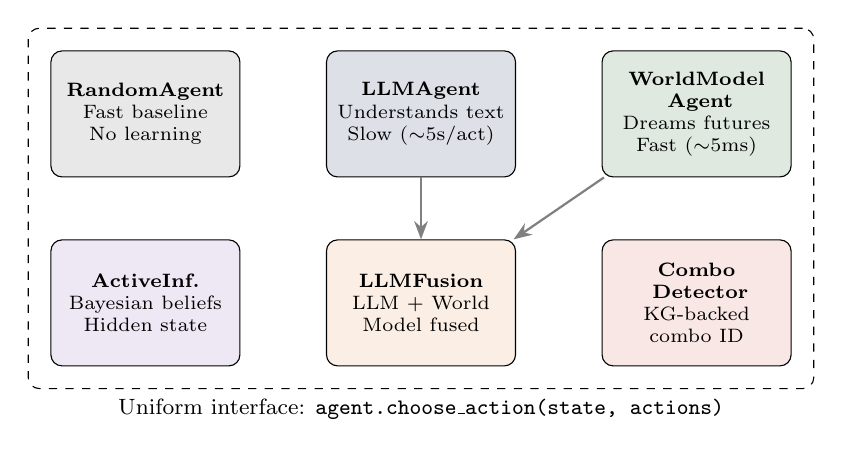
\begin{tikzpicture}[
      every node/.style={font=\scriptsize},
      agent/.style={draw, rounded corners, minimum width=2.4cm, minimum height=1.6cm, align=center},
      >=Stealth,
    ]
    % Row 1
    \node[agent, fill=lightgray] (rand) at (0,0) {\textbf{RandomAgent}\\Fast baseline\\No learning};
    \node[agent, fill=mtgblue!15] (llm) at (3.5,0) {\textbf{LLMAgent}\\Understands text\\Slow ($\sim$5s/act)};
    \node[agent, fill=mtggreen!15] (wma) at (7,0) {\textbf{WorldModel}~\\~\textbf{Agent}\\Dreams futures\\Fast ($\sim$5ms)};
    % Row 2
    \node[agent, fill=kgpurple!12] (active) at (0,-2.4) {\textbf{ActiveInf.}\\Bayesian beliefs\\Hidden state};
    \node[agent, fill=jepaorange!12] (fusion) at (3.5,-2.4) {\textbf{LLMFusion}\\LLM + World\\Model fused};
    \node[agent, fill=mtgred!12] (combo) at (7,-2.4) {\textbf{Combo}~\\~\textbf{Detector}\\KG-backed\\combo ID};

    % Uniform interface
    \node[draw, dashed, rounded corners, fit=(rand)(llm)(wma)(active)(fusion)(combo),
          inner sep=8pt, label={[font=\footnotesize]below:Uniform interface: \texttt{agent.choose\_action(state, actions)}}] {};

    \draw[->, thick, gray] (llm) -- (fusion);
    \draw[->, thick, gray] (wma) -- (fusion);
  \end{tikzpicture}
  \vspace{0.3cm}

  Any agent can play against any other $\Rightarrow$ tournaments, ELO ratings, architecture comparison.
\end{frame}

% -- Slide 6 --------------------------------------------------------
\begin{frame}{The World Model: Imagination as Strategy}
  \begin{center}
  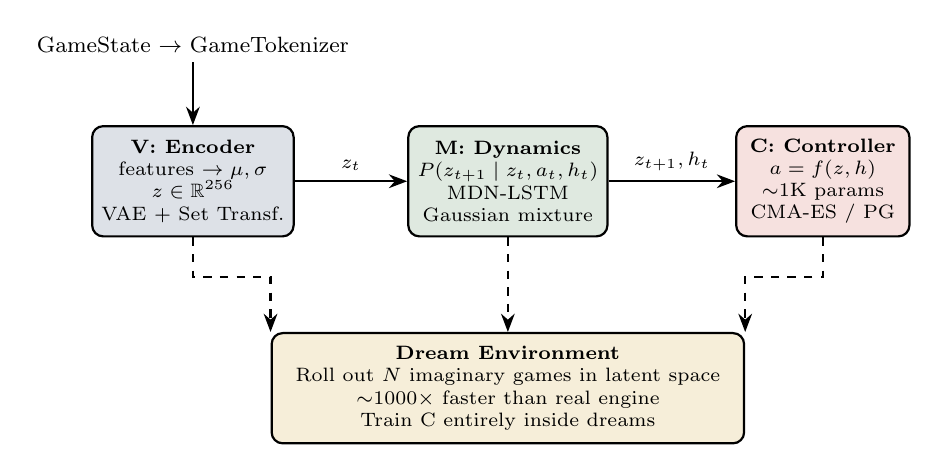
\begin{tikzpicture}[
      every node/.style={font=\scriptsize},
      block/.style={draw, rounded corners, minimum width=2.2cm, minimum height=1.4cm, align=center, thick},
      >=Stealth,
    ]
    % V M C
    \node[block, fill=mtgblue!15] (V) at (0,0) {\textbf{V: Encoder}\\features $\to \mu, \sigma$\\$z \in \mathbb{R}^{256}$\\VAE + Set Transf.};
    \node[block, fill=mtggreen!15] (M) at (4,0) {\textbf{M: Dynamics}\\$P(z_{t+1} \mid z_t, a_t, h_t)$\\MDN-LSTM\\Gaussian mixture};
    \node[block, fill=mtgred!15] (C) at (8,0) {\textbf{C: Controller}\\$a = f(z, h)$\\$\sim$1K params\\CMA-ES / PG};

    % Input
    \node[above=0.8cm of V, font=\footnotesize] (input) {GameState $\to$ GameTokenizer};
    \draw[->, thick] (input) -- (V);

    % Connections
    \draw[->, thick] (V) -- (M) node[midway, above] {$z_t$};
    \draw[->, thick] (M) -- (C) node[midway, above] {$z_{t+1}, h_t$};

    % Dream
    \node[block, fill=mtggold!20, minimum width=6cm, below=1.2cm of M] (dream)
      {\textbf{Dream Environment}\\Roll out $N$ imaginary games in latent space\\$\sim$1000$\times$ faster than real engine\\Train C entirely inside dreams};

    \draw[->, thick, dashed] (V.south) -- ++(0,-0.5) -| (dream.north west);
    \draw[->, thick, dashed] (M.south) -- (dream.north);
    \draw[->, thick, dashed] (C.south) -- ++(0,-0.5) -| (dream.north east);
  \end{tikzpicture}
  \end{center}
  \vspace{0.2cm}
  \textbf{Key:} Controller trains entirely inside dreams --- agent imagines games,
  evaluates policy, improves. No real games needed for controller optimization.
\end{frame}

% -- Slide 7 --------------------------------------------------------
\begin{frame}{Training: Self-Play $\to$ Dream $\to$ Deploy}
  \begin{center}
  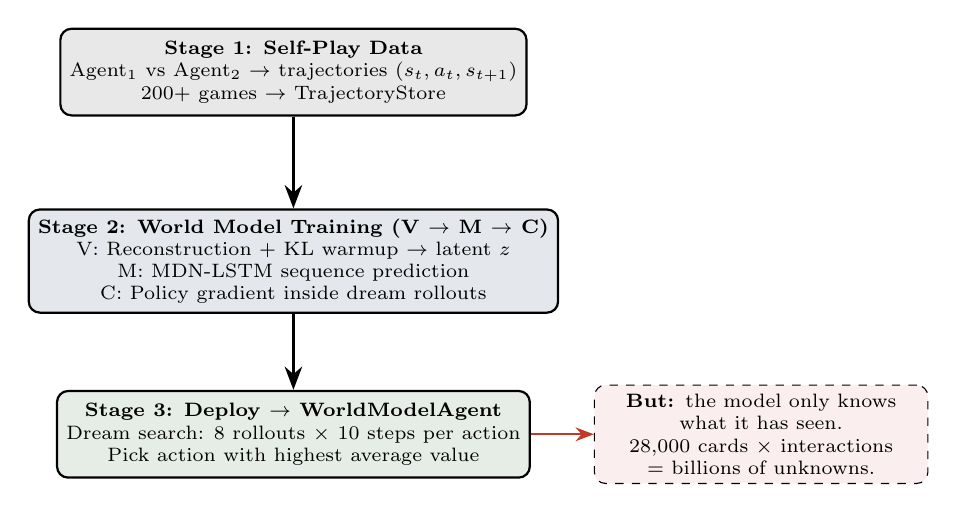
\begin{tikzpicture}[
      every node/.style={font=\scriptsize},
      stage/.style={draw, rounded corners, fill=#1, minimum width=4.5cm, minimum height=1.1cm, align=center, thick},
      >=Stealth,
    ]
    \node[stage=lightgray] (s1) at (0, 2.4)
      {\textbf{Stage 1: Self-Play Data}\\%
       Agent$_1$ vs Agent$_2$ $\to$ trajectories $(s_t, a_t, s_{t+1})$\\%
       200+ games $\to$ TrajectoryStore};

    \node[stage=mtgblue!12] (s2) at (0, 0)
      {\textbf{Stage 2: World Model Training (V $\to$ M $\to$ C)}\\%
       V: Reconstruction + KL warmup $\to$ latent $z$\\%
       M: MDN-LSTM sequence prediction\\%
       C: Policy gradient inside dream rollouts};

    \node[stage=mtggreen!12] (s3) at (0, -2.2)
      {\textbf{Stage 3: Deploy $\to$ WorldModelAgent}\\%
       Dream search: 8 rollouts $\times$ 10 steps per action\\%
       Pick action with highest average value};

    \draw[->, very thick] (s1) -- (s2);
    \draw[->, very thick] (s2) -- (s3);

    % Annotation
    \node[draw, dashed, rounded corners, fill=mtgred!8, text width=4cm, align=center,
          right=0.8cm of s3, font=\scriptsize]
      (limit) {\textbf{But:} the model only knows\\what it has seen.\\28,000 cards $\times$ interactions\\$=$ billions of unknowns.};
    \draw[->, thick, mtgred] (s3.east) -- (limit.west);
  \end{tikzpicture}
  \end{center}
\end{frame}

% -- Slide 8 --------------------------------------------------------
\begin{frame}[fragile]{The Limitation: Knows Only What It Has Seen}
  \begin{columns}[T]
    \begin{column}{0.55\textwidth}
      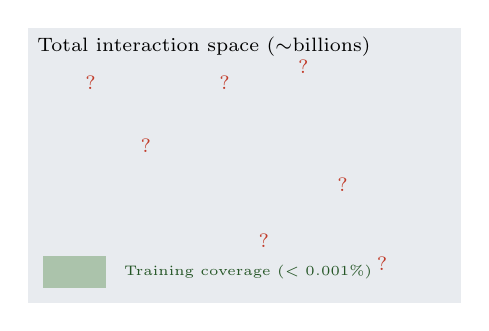
\begin{tikzpicture}[
          every node/.style={font=\scriptsize},
        ]
        % Coverage visualization
        \fill[mtgblue!10] (0,0) rectangle (5.5, 3.5);
        \fill[mtggreen!40] (0.2, 0.2) rectangle (1.0, 0.6);
        \node[font=\scriptsize, anchor=north west] at (0,3.5) {Total interaction space ($\sim$billions)};
        \node[font=\tiny, anchor=west, mtggreen!80!black] at (1.1, 0.4) {Training coverage ($<0.001\%$)};

        % Question marks
        \foreach \x/\y in {2.5/2.8, 4.0/1.5, 1.5/2.0, 3.5/3.0, 4.5/0.5, 0.8/2.8, 3.0/0.8} {
          \node[font=\scriptsize, mtgred] at (\x, \y) {?};
        }
      \end{tikzpicture}
    \end{column}
    \begin{column}{0.42\textwidth}
      \textbf{New card set releases:}
      \begin{itemize}\small
        \item 200+ new cards every 3 months
        \item All interactions are novel
        \item World model is immediately stale
      \end{itemize}
      \vspace{0.3cm}
      \textbf{Commander (singleton):}
      \begin{itemize}\small
        \item 100-card decks, no repeats
        \item Almost nothing seen in training
        \item Dynamics model can't generalize
      \end{itemize}
    \end{column}
  \end{columns}
  \vspace{0.4cm}
  \begin{center}
    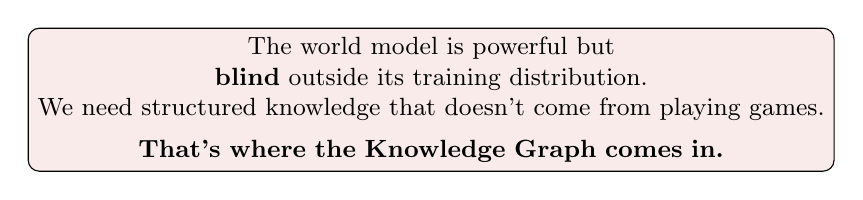
\begin{tikzpicture}
      \node[draw, rounded corners, fill=mtgred!10, text width=10cm, align=center, font=\small] {
        The world model is powerful but \textbf{blind} outside its training distribution.\\
        We need structured knowledge that doesn't come from playing games.\\[4pt]
        \textbf{That's where the Knowledge Graph comes in.}
      };
    \end{tikzpicture}
  \end{center}
\end{frame}


% ===================================================================
\section{Part II --- Why a Knowledge Graph?}
% ===================================================================

% -- Slide 9 --------------------------------------------------------
\begin{frame}{The Central Claim}
  \begin{center}
    \Large
    \begin{quote}
      A world model without a knowledge graph is like a\\
      chess grandmaster with amnesia.\\[6pt]
      \normalsize They can see the board, they can calculate ten moves ahead ---\\
      but they can't remember that bishops move diagonally.
    \end{quote}
  \end{center}
  \vspace{0.5cm}
  \begin{itemize}
    \item World models = powerful \textbf{simulation engines}
    \item Knowledge graphs = powerful \textbf{semantic memories}
    \item Together: full spectrum of intelligent play
  \end{itemize}
\end{frame}

% -- Slide 10 -------------------------------------------------------
\begin{frame}{What World Models Do Well}
  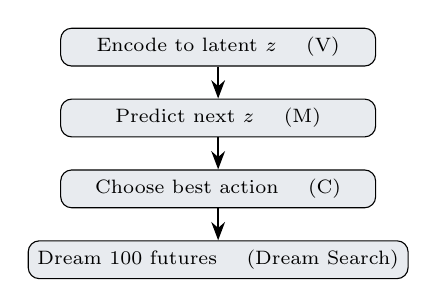
\begin{tikzpicture}[
      every node/.style={font=\scriptsize},
      stepbox/.style={draw, rounded corners, fill=mtgblue!10, minimum width=4cm, align=center},
      >=Stealth,
    ]
    \node[stepbox] (enc) at (0, 0) {Encode to latent $z$ \quad (V)};
    \node[stepbox] (pred) at (0, -0.9) {Predict next $z$ \quad (M)};
    \node[stepbox] (act) at (0, -1.8) {Choose best action \quad (C)};
    \node[stepbox] (dream) at (0, -2.7) {Dream 100 futures \quad (Dream Search)};

    \draw[->, thick] (enc) -- (pred);
    \draw[->, thick] (pred) -- (act);
    \draw[->, thick] (act) -- (dream);
  \end{tikzpicture}
  \hfill
  \begin{minipage}[t]{0.5\textwidth}
    \textbf{Strengths:}
    \begin{itemize}
      \item Imagine future states without running the rules engine
      \item Learn opponent behavior patterns from games
      \item Long-horizon planning in latent space
      \item Train \textit{inside the dream} --- no real environment needed
    \end{itemize}
    \vspace{0.3cm}
    \textbf{The magic number:}\\
    Dream search $\approx$ 1000$\times$ faster than real engine.
  \end{minipage}
\end{frame}

% -- Slide 11 -------------------------------------------------------
\begin{frame}{What World Models Struggle With}
  \begin{table}
    \centering\small
    \begin{tabular}{@{}lp{7cm}@{}}
      \toprule
      \textbf{Problem} & \textbf{Why It Hurts} \\
      \midrule
      Novel cards & Dynamics model never saw the new set \\
      Combinatorial explosion & 28,000 cards $\times$ $N$ interactions \\
      Rule edge cases & Layers, replacement effects, split-second \\
      Explainability & Latent trajectory says nothing meaningful \\
      Format transfer & Standard $\to$ Commander requires restart \\
      Sample efficiency & Must \textit{see} each interaction many times \\
      \bottomrule
    \end{tabular}
  \end{table}
  \vspace{0.5cm}
  \begin{center}
    \textbf{Core tension:} World models learn by doing.\\
    Knowledge graphs know by construction.
  \end{center}
\end{frame}

% -- Slide 12 -------------------------------------------------------
\begin{frame}{What a Knowledge Graph Knows}
  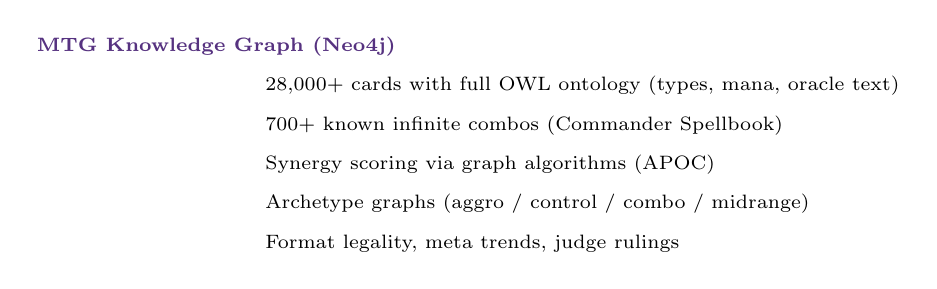
\begin{tikzpicture}[
      every node/.style={font=\scriptsize},
      branch/.style={draw=none, text=kgpurple!80!black, font=\scriptsize\bfseries},
      leaf/.style={draw=none, font=\scriptsize},
    ]
    \node[branch] (root) at (0,0) {MTG Knowledge Graph (Neo4j)};
    \node[leaf, anchor=west] at (0.5, -0.5) {28,000+ cards with full OWL ontology (types, mana, oracle text)};
    \node[leaf, anchor=west] at (0.5, -1.0) {700+ known infinite combos (Commander Spellbook)};
    \node[leaf, anchor=west] at (0.5, -1.5) {Synergy scoring via graph algorithms (APOC)};
    \node[leaf, anchor=west] at (0.5, -2.0) {Archetype graphs (aggro / control / combo / midrange)};
    \node[leaf, anchor=west] at (0.5, -2.5) {Format legality, meta trends, judge rulings};
  \end{tikzpicture}
  \vspace{0.5cm}

  This knowledge is \textbf{complete, correct, and permanent}.

  It doesn't need training games to learn that Thassa's Oracle wins on an empty library. It already knows.
\end{frame}

% -- Slide 13 -------------------------------------------------------
\begin{frame}{The Complementarity: System 1 + System 2}
  \begin{center}
  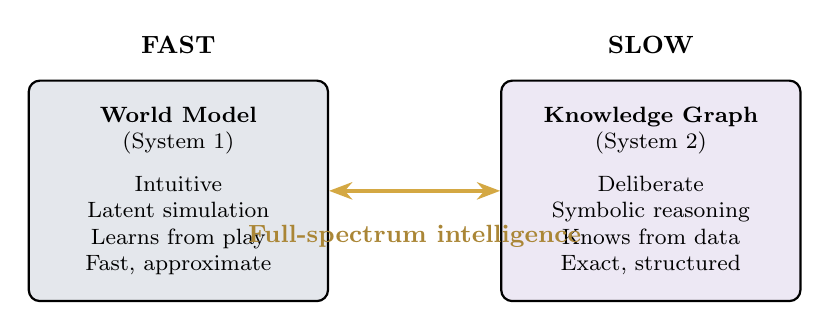
\begin{tikzpicture}[
      every node/.style={font=\footnotesize},
      sysbox/.style={draw, thick, rounded corners, minimum width=3.8cm, minimum height=2.8cm, align=center},
      >=Stealth,
    ]
    % System 1
    \node[sysbox, fill=mtgblue!12] (s1) at (0,0) {%
      \textbf{World Model}\\(System 1)\\[6pt]
      Intuitive\\Latent simulation\\Learns from play\\Fast, approximate};

    % System 2
    \node[sysbox, fill=kgpurple!12] (s2) at (6,0) {%
      \textbf{Knowledge Graph}\\(System 2)\\[6pt]
      Deliberate\\Symbolic reasoning\\Knows from data\\Exact, structured};

    % Labels
    \node[above=0.2cm of s1, font=\small\bfseries] {FAST};
    \node[above=0.2cm of s2, font=\small\bfseries] {SLOW};

    % Arrow
    \draw[{Stealth}-{Stealth}, very thick, mtggold] (s1.east) -- (s2.west)
      node[midway, below=0.3cm, font=\small\bfseries, mtggold!80!black] {Full-spectrum intelligence};
  \end{tikzpicture}
  \end{center}
  \vspace{0.3cm}
  \begin{center}
    \textit{Kahneman applied to game AI}: neither alone is sufficient.
  \end{center}
\end{frame}

% -- Slide 14 -------------------------------------------------------
\begin{frame}{Benefit 1: Semantic Grounding}
  \textbf{Problem:} $z \in \mathbb{R}^{256}$ means nothing. Dimension 47 might be ``mana advantage'' --- or not.

  \vspace{0.3cm}
  \textbf{KG solution:} Initialize card embeddings from KG node features.
  \vspace{0.2cm}

  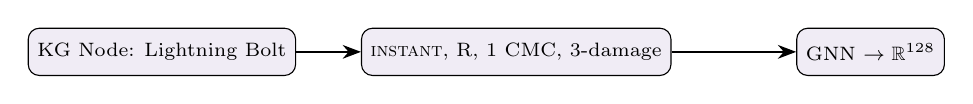
\begin{tikzpicture}[
      every node/.style={font=\scriptsize},
      stepbox/.style={draw, rounded corners, fill=kgpurple!10, minimum height=0.6cm, align=center},
      >=Stealth,
    ]
    \node[stepbox] (kg) at (0,0) {KG Node: Lightning Bolt};
    \node[stepbox] (feat) at (4.5,0) {\textsc{instant}, R, 1 CMC, 3-damage};
    \node[stepbox] (gnn) at (9,0) {GNN $\to \mathbb{R}^{128}$};

    \draw[->, thick] (kg) -- (feat);
    \draw[->, thick] (feat) -- (gnn);
  \end{tikzpicture}

  \vspace{0.4cm}
  \textbf{Result:} Latent space \textit{starts structured} --- directions correspond to:
  \begin{itemize}
    \item Tempo vs.\ card advantage axis
    \item Aggro vs.\ control positioning
    \item Board presence vs.\ resource accumulation
  \end{itemize}
  \vspace{0.2cm}
  Training convergence improves dramatically.
\end{frame}

% -- Slide 15 -------------------------------------------------------
\begin{frame}{Benefit 2: Zero-Shot Reasoning About New Cards}
  \textbf{Problem:} New set releases. World model has never seen these cards.

  \vspace{0.3cm}
  \begin{columns}[T]
    \begin{column}{0.48\textwidth}
      \textbf{Without KG:}\\
      Agent misplays new cards for weeks until enough training games are collected.
    \end{column}
    \begin{column}{0.48\textwidth}
      \textbf{With KG:}\\
      New set imported into Neo4j overnight.\\
      KG provides the \textit{prior} that bootstraps reasoning.\\
      World model only needs a handful of games to \textit{calibrate}.
    \end{column}
  \end{columns}

  \vspace{0.5cm}
  \textbf{Zero-shot combo detection:}
  If two new cards form a loop, the KG detects it via graph traversal \textit{before the agent ever plays them}.
\end{frame}

% -- Slide 16 -------------------------------------------------------
\begin{frame}{Benefit 3: Opponent Modeling Beyond Statistics}
  A pure world model learns opponent behavior as a distribution over actions.\\
  Good --- but it misses \textit{intent}.

  \vspace{0.3cm}
  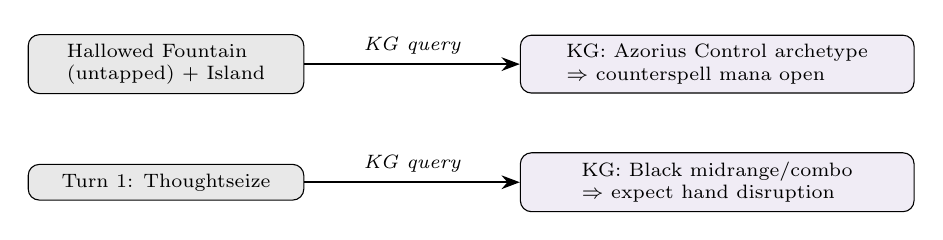
\begin{tikzpicture}[
      every node/.style={font=\scriptsize},
      obs/.style={draw, rounded corners, fill=lightgray, minimum width=3.5cm, align=left},
      inf/.style={draw, rounded corners, fill=kgpurple!10, minimum width=5cm, align=left},
      >=Stealth,
    ]
    \node[obs] (o1) at (0, 0) {Hallowed Fountain\\(untapped) + Island};
    \node[inf] (i1) at (7, 0) {KG: Azorius Control archetype\\$\Rightarrow$ counterspell mana open};
    \draw[->, thick] (o1) -- (i1) node[midway, above, font=\scriptsize\itshape] {KG query};

    \node[obs] (o2) at (0, -1.5) {Turn 1: Thoughtseize};
    \node[inf] (i2) at (7, -1.5) {KG: Black midrange/combo\\$\Rightarrow$ expect hand disruption};
    \draw[->, thick] (o2) -- (i2) node[midway, above, font=\scriptsize\itshape] {KG query};
  \end{tikzpicture}

  \vspace{0.4cm}
  The KG doesn't just say ``opponent will likely pass'' ---\\
  it says \textbf{why} and \textbf{what comes next}.\\[4pt]
  This is the difference between \textit{correlation} and \textit{causal structure}.
\end{frame}

% -- Slide 17 -------------------------------------------------------
\begin{frame}{Benefit 4: Sample Efficiency $\times$ 10}
  \begin{columns}[T]
    \begin{column}{0.55\textwidth}
      \textbf{Without KG:}\\
      Must \textit{discover} that Lightning Bolt deals 3 damage.\\
      200 similar cards --- each learned separately.\\
      $\sim$100{,}000 games per interaction.
      \vspace{0.3cm}

      \textbf{With KG:}\\
      KG groups 47 cards that deal 3 damage.\\
      Shared embedding in feature space.\\
      Seeing \textit{any one} generalizes to all.
    \end{column}
    \begin{column}{0.42\textwidth}
      \begin{table}
        \centering\scriptsize
        \begin{tabular}{@{}lc@{}}
          \toprule
          \textbf{Scenario} & \textbf{Games} \\
          \midrule
          Pure WM & $O(N \cdot s)$ \\
          WM + KG & $O(C \cdot s)$ \\
          \bottomrule
        \end{tabular}
      \end{table}
      \vspace{0.2cm}
      \footnotesize
      $C$ (clusters) $\ll$ $N$ (interactions).\\
      Orders of magnitude fewer games.
    \end{column}
  \end{columns}
\end{frame}

% -- Slide 18 -------------------------------------------------------
\begin{frame}{Benefit 5: Closing the Explainability Gap}
  \textbf{Problem:} Dream search evaluated 500 futures. Result: ``action 7 had highest value.''

  \vspace{0.3cm}
  \textbf{KG-augmented explanation:}
  \begin{enumerate}\small
    \item Dream search found: \textit{Play Goblin Charbelcher, activate for 12 (lethal)}
    \item KG lookup: No lands in deck $\Rightarrow$ Charbelcher deals cards-until-land damage
    \item KG: This is the ``Belcher'' combo --- known goldfish deck
    \item Explanation: \textit{``Agent held Force of Will, countering Charbelcher activation.''}
  \end{enumerate}

  \vspace{0.3cm}
  Matters for:
  \begin{itemize}
    \item \textbf{Trust} --- humans coaching the system need to understand decisions
    \item \textbf{Debugging} --- identifying hallucinated illegal lines
    \item \textbf{Education} --- teaching new players correct reasoning
  \end{itemize}
\end{frame}

% -- Slide 19 -------------------------------------------------------
\begin{frame}{Benefit 6: Format Transfer Without Retraining}
  Standard $\to$ Pioneer $\to$ Modern $\to$ Legacy $\to$ Commander
  \vspace{0.3cm}

  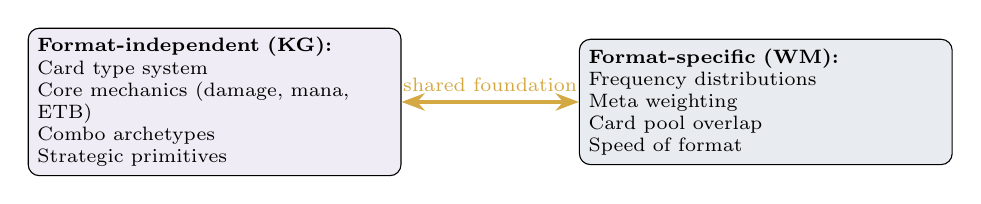
\begin{tikzpicture}[
      every node/.style={font=\scriptsize},
      const/.style={draw, rounded corners, fill=kgpurple!10, text width=4.5cm, align=left},
      var/.style={draw, rounded corners, fill=mtgblue!10, text width=4.5cm, align=left},
      >=Stealth,
    ]
    \node[const] (c) at (0,0) {\textbf{Format-independent (KG):}\\
      Card type system\\
      Core mechanics (damage, mana, ETB)\\
      Combo archetypes\\
      Strategic primitives};
    \node[var] (v) at (7, 0) {\textbf{Format-specific (WM):}\\
      Frequency distributions\\
      Meta weighting\\
      Card pool overlap\\
      Speed of format};

    \draw[{Stealth}-{Stealth}, very thick, mtggold] (c.east) -- (v.west)
      node[midway, above, font=\scriptsize] {shared foundation};
  \end{tikzpicture}

  \vspace{0.4cm}
  Commander = 100-card singleton? The KG still knows every card.\\
  The dynamics model just learns \textit{frequency distributions} change.
\end{frame}

% -- Slide 20 -------------------------------------------------------
\begin{frame}{The Three Memory Systems Together}
  \begin{center}
  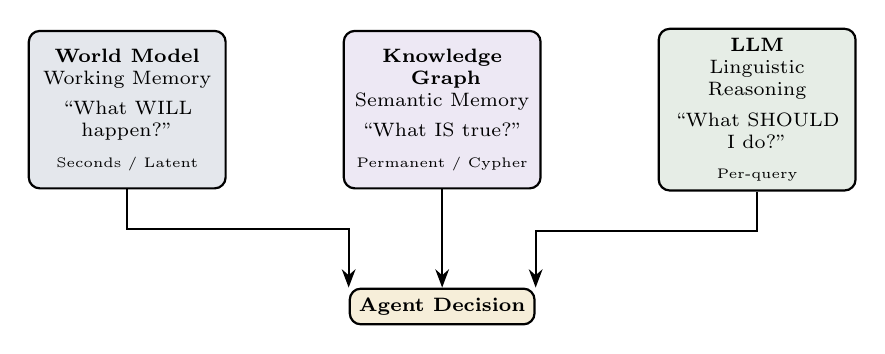
\begin{tikzpicture}[
      every node/.style={font=\scriptsize},
      mem/.style={draw, thick, rounded corners, minimum width=2.5cm, minimum height=2cm, align=center},
      >=Stealth,
    ]
    \node[mem, fill=mtgblue!12] (wm) at (0,0) {\textbf{World Model}\\Working Memory\\[3pt]``What WILL\\happen?''\\[3pt]\tiny Seconds / Latent};
    \node[mem, fill=kgpurple!12] (kg) at (4,0) {\textbf{Knowledge}\\~\textbf{Graph}\\Semantic Memory\\[3pt]``What IS true?''\\[3pt]\tiny Permanent / Cypher};
    \node[mem, fill=mtggreen!12] (llm) at (8,0) {\textbf{LLM}\\Linguistic\\Reasoning\\[3pt]``What SHOULD\\I do?''\\[3pt]\tiny Per-query};

    % Decision node
    \node[draw, thick, fill=mtggold!20, rounded corners, minimum width=1.5cm] (dec) at (4, -2.5) {\textbf{Agent Decision}};

    \draw[->, thick] (wm.south) -- ++(0,-0.5) -| (dec.north west);
    \draw[->, thick] (kg.south) -- (dec.north);
    \draw[->, thick] (llm.south) -- ++(0,-0.5) -| (dec.north east);
  \end{tikzpicture}
  \end{center}
  \vspace{0.2cm}
  \begin{table}
    \centering\scriptsize
    \begin{tabular}{@{}lll@{}}
      \toprule
      \textbf{Memory} & \textbf{Cognitive Analog} & \textbf{When Consulted} \\
      \midrule
      World Model & Hippocampus       & Every action (fast path) \\
      Knowledge Graph & Neocortex     & Novel situations, combos, opponent profiling \\
      LLM         & Prefrontal cortex & Strategic pivots, ambiguous rules \\
      \bottomrule
    \end{tabular}
  \end{table}
\end{frame}

% -- Slide 21 -------------------------------------------------------
\begin{frame}[fragile]{Concrete Integration Points}
  \begin{lstlisting}[language=Python]
# 1. Card embeddings initialized from KG features
card_emb = kg.get_card_embedding("Lightning Bolt")  # GNN over KG
tokenizer = GameTokenizer(card_embeddings=card_emb)  # feeds V

# 2. KG-conditioned opponent model
archetype = kg.classify_opponent_archetype(observed_plays)
world_model.update_opponent_prior(archetype)         # conditions M

# 3. Combo-aware reward signal
combos = kg.detect_available_combos(game_state)
reward = base_reward + kg_combo_bonus(combos)         # shapes C

# 4. KG as fallback for novel states
if world_model.uncertainty(z) > threshold:
    ruling = kg.get_interaction_ruling(cards_in_play)
    action = rule_based_override(ruling)

# 5. Post-hoc explanation
dream_trace = world_model.last_dream_trace()
explanation = kg.explain_trajectory(dream_trace)
  \end{lstlisting}
\end{frame}

% -- Slide 22 -------------------------------------------------------
\begin{frame}{Summary: The Synergy Argument}
  \begin{columns}[T]
    \begin{column}{0.48\textwidth}
      \textbf{Problem:}
      \begin{itemize}\small
        \item WMs are empirical --- know what they've seen
        \item 28,000 cards $\times$ exponential interactions
        \item No agent sees enough games
      \end{itemize}
      \vspace{0.3cm}
      \textbf{Solution:}
      \begin{itemize}\small
        \item KG provides top-down symbolic structure
        \item WM provides bottom-up experiential learning
        \item They meet in the middle: \textbf{structured latent space}
      \end{itemize}
    \end{column}
    \begin{column}{0.48\textwidth}
      \textbf{Result:}
      \begin{itemize}\small
        \item[\checkmark] Faster convergence
        \item[\checkmark] Zero-shot generalization
        \item[\checkmark] Richer opponent models
        \item[\checkmark] Explainable decisions
        \item[\checkmark] Format transfer
        \item[\checkmark] 10$\times$ sample efficiency
      \end{itemize}
      \vspace{0.3cm}
      \begin{center}
        \textit{The KG does not replace the WM.\\
        It tells the WM what it is\\allowed to imagine.}
      \end{center}
    \end{column}
  \end{columns}
\end{frame}


% ===================================================================
\section{Part III --- JEPA / LeWM}
% ===================================================================

% -- Slide 23 -------------------------------------------------------
\begin{frame}{What Is LeWM?}
  \footnotesize
  \textbf{Paper:} Maes et al.\ (2026). ``LeWorldModel: Stable End-to-End JEPA from Pixels.''
  arXiv:2603.19312\\
  \textbf{Code:} \texttt{github.com/lucas-maes/le-wm} \quad
  \textbf{JEPA} = Joint Embedding Predictive Architecture

  \vspace{0.4cm}
  \begin{center}
  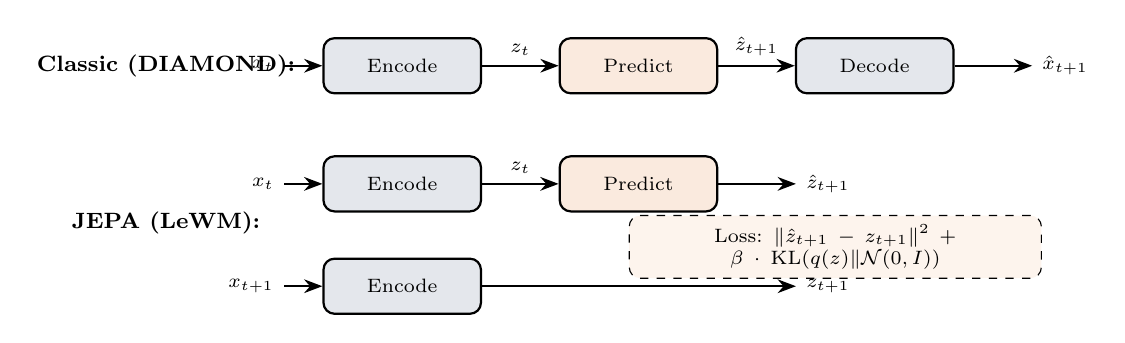
\begin{tikzpicture}[
      every node/.style={font=\scriptsize},
      enc/.style={draw, thick, rounded corners, fill=mtgblue!12, minimum width=2cm, minimum height=0.7cm, align=center},
      pred/.style={draw, thick, rounded corners, fill=jepaorange!15, minimum width=2cm, minimum height=0.7cm, align=center},
      >=Stealth,
    ]
    % Classic
    \node[font=\footnotesize\bfseries] at (-1, 2) {Classic (DIAMOND):};
    \node[enc] (e1) at (2, 2) {Encode};
    \node[pred] (p1) at (5, 2) {Predict};
    \node[enc] (d1) at (8, 2) {Decode};
    \draw[->, thick] (0.5, 2) node[left] {$x_t$} -- (e1);
    \draw[->, thick] (e1) -- (p1) node[midway, above] {$z_t$};
    \draw[->, thick] (p1) -- (d1) node[midway, above] {$\hat{z}_{t+1}$};
    \draw[->, thick] (d1) -- (10, 2) node[right] {$\hat{x}_{t+1}$};

    % JEPA
    \node[font=\footnotesize\bfseries] at (-1, 0) {JEPA (LeWM):};
    \node[enc] (e2a) at (2, 0.5) {Encode};
    \node[pred] (p2) at (5, 0.5) {Predict};
    \node[enc] (e2b) at (2, -0.8) {Encode};
    \draw[->, thick] (0.5, 0.5) node[left] {$x_t$} -- (e2a);
    \draw[->, thick] (e2a) -- (p2) node[midway, above] {$z_t$};
    \draw[->, thick] (0.5, -0.8) node[left] {$x_{t+1}$} -- (e2b);
    \draw[->, thick] (p2) -- ++(2.0, 0) node[right] {$\hat{z}_{t+1}$};
    \draw[->, thick] (e2b) -- ++(5.0, 0) node[right] {$z_{t+1}$};

    % Loss
    \node[draw, dashed, rounded corners, fill=jepaorange!8, text width=5cm, align=center] at (7.5, -0.3)
      {Loss: $\|\hat{z}_{t+1} - z_{t+1}\|^2 + \beta \cdot \mathrm{KL}(q(z) \| \mathcal{N}(0,I))$};
  \end{tikzpicture}
  \end{center}
  \vspace{0.2cm}
  \begin{itemize}
    \item No decoder needed --- predict in latent space directly
    \item Gaussian regularizer prevents collapse (no EMA, no stop-grad on targets needed)
    \item \textbf{One hyperparameter:} $\beta$
  \end{itemize}
\end{frame}

% -- Slide 24 -------------------------------------------------------
\begin{frame}{LeWM Numbers That Matter}
  \begin{table}
    \centering\small
    \begin{tabular}{@{}lccc@{}}
      \toprule
      \textbf{Metric} & \textbf{LeWM} & \textbf{Foundation WM} & \textbf{DIAMOND} \\
      \midrule
      Parameters       & $\sim$15M     & $\sim$1B+              & 4.4M--381M \\
      Training         & 1 GPU, hours  & Multi-GPU, days        & Multi-GPU, days \\
      Planning speed   & Baseline      & \textbf{48$\times$ slower}  & Faster \\
      Loss terms       & \textbf{2}    & 6--8                   & 3--4 \\
      Hyperparameters  & \textbf{1}    & 5--7                   & 3--5 \\
      Collapse avoid.  & Gaussian reg. & EMA + stop-grad        & VQ-VAE \\
      Latent structure & \textbf{Physical} & Unclear             & Discrete tokens \\
      \bottomrule
    \end{tabular}
  \end{table}
  \vspace{0.3cm}
  \textbf{Key insight:} LeWM's latent space provably encodes physical/semantic structure (confirmed by probing).\\
  This is exactly what we need for a structured game like MTG.
\end{frame}

% -- Slide 25 -------------------------------------------------------
\begin{frame}{Why JEPA Fits MTG Better Than Pixel Diffusion}
  Our game state is structured data, not pixels:

  \vspace{0.2cm}
  \begin{table}
    \centering\footnotesize
    \begin{tabular}{@{}llll@{}}
      \toprule
      \textbf{Property} & \textbf{DIAMOND} & \textbf{JEPA} & \textbf{MTG Fit} \\
      \midrule
      Input type        & Pixels          & Any embeddable     & \checkmark\ Structured state \\
      Prediction target & Pixel space     & Latent space       & \checkmark\ Latent game state \\
      Semantic struct.  & Lost in pixels  & Encoded in $z$     & \checkmark\ KG preserves meaning \\
      Physical probing  & N/A             & Confirmed          & \checkmark\ Mana, life, cards \\
      Training obj.     & Denoising MSE   & Pred.\ + KL        & \checkmark\ Cleaner \\
      Planning speed    & Slow (denoise)  & 48$\times$ faster  & \checkmark\ More rollouts/turn \\
      \bottomrule
    \end{tabular}
  \end{table}
  \vspace{0.3cm}
  \begin{center}
    \textbf{JEPA is the natural choice for structured-state domains.}
  \end{center}
\end{frame}

% -- Slide 26 -------------------------------------------------------
\begin{frame}{The Surprise Detection Bonus}
  LeWM detects when observed transitions are \textbf{physically implausible}.

  \vspace{0.3cm}
  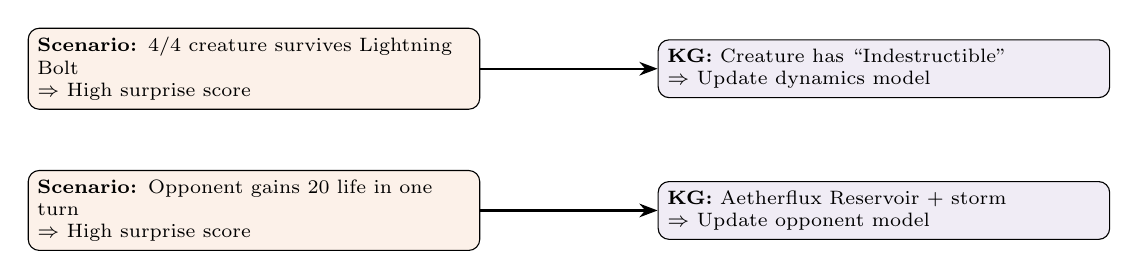
\begin{tikzpicture}[
      every node/.style={font=\scriptsize},
      scenario/.style={draw, rounded corners, fill=jepaorange!10, text width=5.5cm, align=left},
      response/.style={draw, rounded corners, fill=kgpurple!10, text width=5.5cm, align=left},
      >=Stealth,
    ]
    \node[scenario] (s1) at (0, 0) {\textbf{Scenario:} 4/4 creature survives Lightning Bolt\\
      $\Rightarrow$ High surprise score};
    \node[response] (r1) at (8, 0) {\textbf{KG:} Creature has ``Indestructible''\\
      $\Rightarrow$ Update dynamics model};

    \node[scenario] (s2) at (0, -1.8) {\textbf{Scenario:} Opponent gains 20 life in one turn\\
      $\Rightarrow$ High surprise score};
    \node[response] (r2) at (8, -1.8) {\textbf{KG:} Aetherflux Reservoir + storm\\
      $\Rightarrow$ Update opponent model};

    \draw[->, thick] (s1) -- (r1);
    \draw[->, thick] (s2) -- (r2);
  \end{tikzpicture}

  \vspace{0.4cm}
  \textbf{Surprise detection = automatic knowledge gap identification.}\\
  When the world model is wrong, the KG explains why.
\end{frame}

% -- Slide 27 -------------------------------------------------------
\begin{frame}{Dual-Input JEPA Architecture}
  \begin{center}
  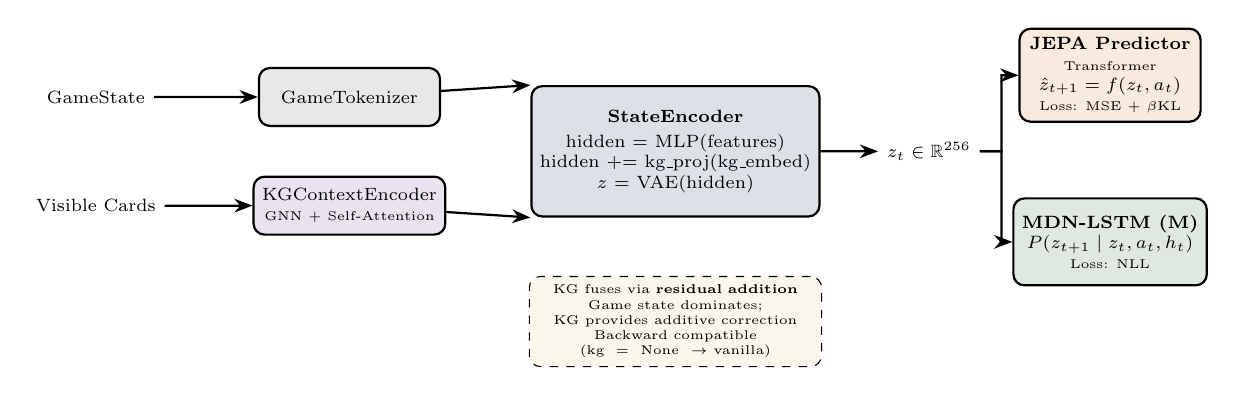
\begin{tikzpicture}[
      every node/.style={font=\scriptsize},
      block/.style={draw, thick, rounded corners, minimum height=0.8cm, align=center},
      >=Stealth, scale=0.92, transform shape,
    ]
    % Inputs
    \node (gs) at (-2, 3.5) {GameState};
    \node (vc) at (-2, 2.0) {Visible Cards};

    % Tokenizer
    \node[block, fill=lightgray, minimum width=2.5cm] (tok) at (1.5, 3.5) {GameTokenizer};
    \draw[->, thick] (gs) -- (tok);

    % KG Encoder
    \node[block, fill=kgpurple!15, minimum width=2.5cm] (kge) at (1.5, 2.0) {KGContextEncoder\\{\tiny GNN + Self-Attention}};
    \draw[->, thick] (vc) -- (kge);

    % StateEncoder
    \node[block, fill=mtgblue!15, minimum width=3.5cm, minimum height=1.8cm] (enc) at (6, 2.75) {
      \textbf{StateEncoder}\\[2pt]
      hidden = MLP(features)\\
      hidden += kg\_proj(kg\_embed)\\
      $z$ = VAE(hidden)};
    \draw[->, thick] (tok) -- (enc.north west);
    \draw[->, thick] (kge) -- (enc.south west);

    % z output
    \node (zt) at (9.5, 2.75) {$z_t \in \mathbb{R}^{256}$};
    \draw[->, thick] (enc) -- (zt);

    % JEPA predictor
    \node[block, fill=jepaorange!15, minimum width=2.5cm, minimum height=1.2cm] (jepa) at (12, 3.8)
      {\textbf{JEPA Predictor}\\{\tiny Transformer}\\$\hat{z}_{t+1} = f(z_t, a_t)$\\{\tiny Loss: MSE + $\beta$KL}};

    % MDN-LSTM
    \node[block, fill=mtggreen!15, minimum width=2.5cm, minimum height=1.2cm] (mdn) at (12, 1.5)
      {\textbf{MDN-LSTM (M)}\\$P(z_{t+1} \mid z_t, a_t, h_t)$\\{\tiny Loss: NLL}};

    \draw[->, thick] (zt) -- ++(1.0, 0) |- (jepa.west);
    \draw[->, thick] (zt) -- ++(1.0, 0) |- (mdn.west);

    % Residual note
    \node[draw, dashed, rounded corners, fill=mtggold!10, text width=3.8cm, font=\tiny, align=center]
      at (6, 0.4) {KG fuses via \textbf{residual addition}\\Game state dominates;\\KG provides additive correction\\Backward compatible ($\text{kg}=\text{None} \to$ vanilla)};
  \end{tikzpicture}
  \end{center}
\end{frame}

% -- Slide 28 -------------------------------------------------------
\begin{frame}[fragile]{LeWM + KG: The Killer Combination}
  \begin{center}
  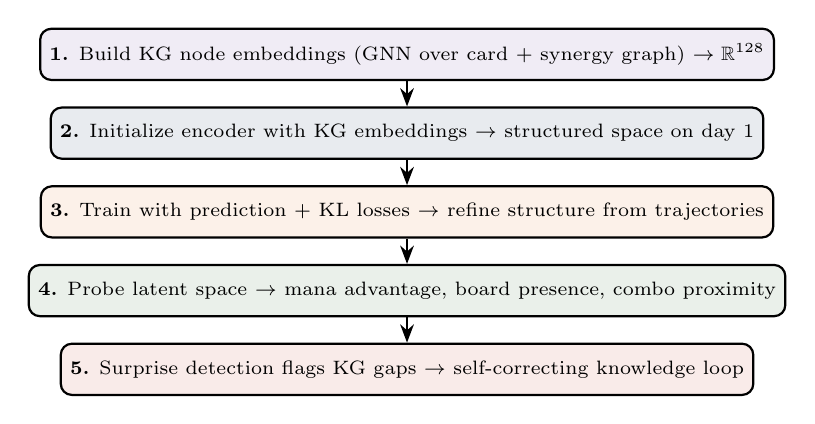
\begin{tikzpicture}[
      every node/.style={font=\scriptsize},
      stepbox/.style={draw, thick, rounded corners, fill=#1, minimum width=8cm, minimum height=0.65cm, align=left},
      >=Stealth,
    ]
    \node[stepbox=kgpurple!10] (s1) at (0, 3)
      {\textbf{1.} Build KG node embeddings (GNN over card + synergy graph) $\to \mathbb{R}^{128}$};
    \node[stepbox=mtgblue!10] (s2) at (0, 2)
      {\textbf{2.} Initialize encoder with KG embeddings $\to$ structured space on day 1};
    \node[stepbox=jepaorange!10] (s3) at (0, 1)
      {\textbf{3.} Train with prediction + KL losses $\to$ refine structure from trajectories};
    \node[stepbox=mtggreen!10] (s4) at (0, 0)
      {\textbf{4.} Probe latent space $\to$ mana advantage, board presence, combo proximity};
    \node[stepbox=mtgred!10] (s5) at (0, -1)
      {\textbf{5.} Surprise detection flags KG gaps $\to$ self-correcting knowledge loop};

    \draw[->, thick] (s1) -- (s2);
    \draw[->, thick] (s2) -- (s3);
    \draw[->, thick] (s3) -- (s4);
    \draw[->, thick] (s4) -- (s5);
  \end{tikzpicture}
  \end{center}
  \vspace{0.3cm}
  \begin{columns}[c]
    \column{0.33\textwidth}\centering Convergence in\\$\sim$10$\times$ fewer games
    \column{0.33\textwidth}\centering Latent dimensions\\are interpretable
    \column{0.33\textwidth}\centering Knowledge gaps\\are self-identified
  \end{columns}
\end{frame}

% -- Slide 29 -------------------------------------------------------
\begin{frame}{Implementation Status}
  \small
  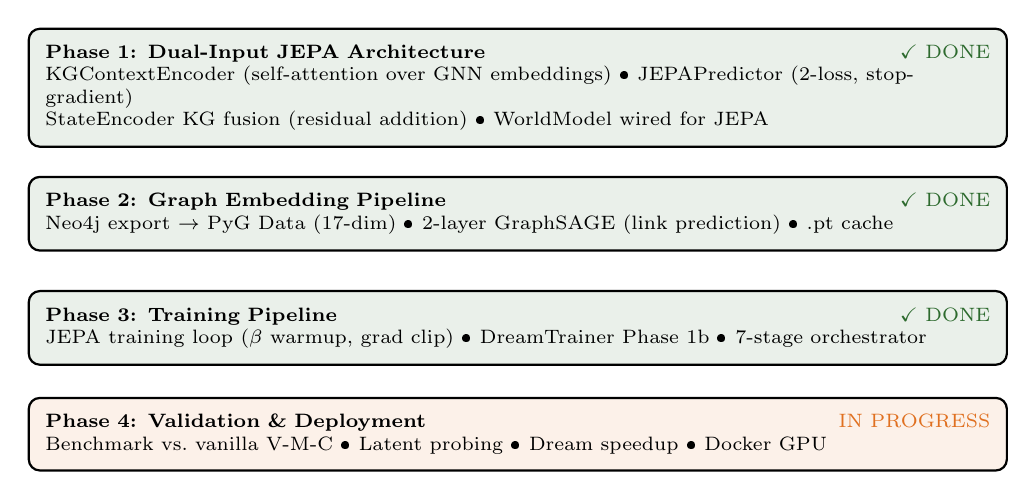
\begin{tikzpicture}[
      every node/.style={font=\scriptsize},
      phase/.style={draw, thick, rounded corners, text width=12cm, align=left, inner sep=6pt},
    ]
    \node[phase, fill=mtggreen!10] (p1) at (0, 2.8)
      {\textbf{Phase 1: Dual-Input JEPA Architecture} \hfill \textcolor{mtggreen}{\checkmark\ DONE}\\
       KGContextEncoder (self-attention over GNN embeddings)
       \textbullet\ JEPAPredictor (2-loss, stop-gradient)\\
       StateEncoder KG fusion (residual addition)
       \textbullet\ WorldModel wired for JEPA};
    \node[phase, fill=mtggreen!10] (p2) at (0, 1.2)
      {\textbf{Phase 2: Graph Embedding Pipeline} \hfill \textcolor{mtggreen}{\checkmark\ DONE}\\
       Neo4j export $\to$ PyG Data (17-dim)
       \textbullet\ 2-layer GraphSAGE (link prediction)
       \textbullet\ .pt cache};
    \node[phase, fill=mtggreen!10] (p3) at (0, -0.25)
      {\textbf{Phase 3: Training Pipeline} \hfill \textcolor{mtggreen}{\checkmark\ DONE}\\
       JEPA training loop ($\beta$ warmup, grad clip)
       \textbullet\ DreamTrainer Phase 1b
       \textbullet\ 7-stage orchestrator};
    \node[phase, fill=jepaorange!10] (p4) at (0, -1.6)
      {\textbf{Phase 4: Validation \& Deployment} \hfill \textcolor{jepaorange}{IN PROGRESS}\\
       Benchmark vs.\ vanilla V-M-C
       \textbullet\ Latent probing
       \textbullet\ Dream speedup
       \textbullet\ Docker GPU};
  \end{tikzpicture}
\end{frame}

% -- Slide 30 -------------------------------------------------------
\begin{frame}{Final Thesis}
  \begin{center}
    \large\bfseries World Model + Knowledge Graph + JEPA\\= a genuinely novel agent architecture
  \end{center}
  \vspace{0.3cm}
  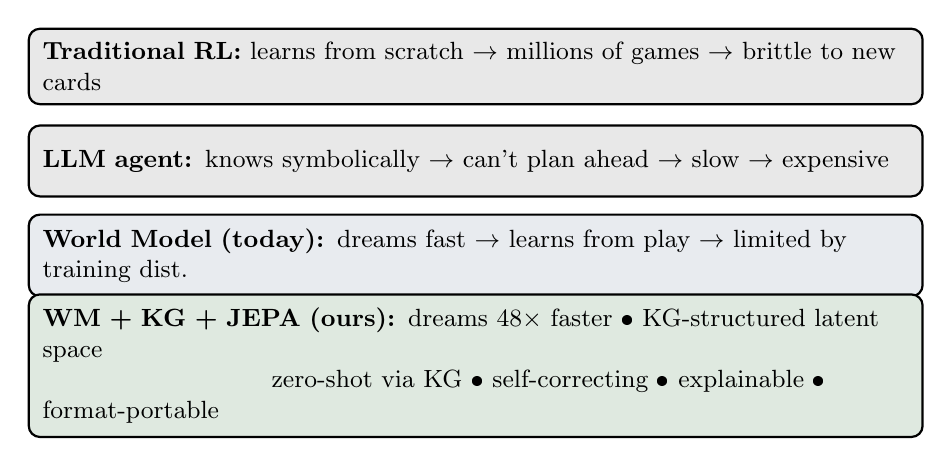
\begin{tikzpicture}[
      every node/.style={font=\small},
      row/.style={draw, thick, rounded corners, text width=11cm, align=left, minimum height=0.9cm, inner sep=5pt},
    ]
    \node[row, fill=lightgray] at (0, 2.4)
      {\textbf{Traditional RL:} learns from scratch $\to$ millions of games $\to$ brittle to new cards};
    \node[row, fill=lightgray] at (0, 1.2)
      {\textbf{LLM agent:} knows symbolically $\to$ can't plan ahead $\to$ slow $\to$ expensive};
    \node[row, fill=mtgblue!10] at (0, 0)
      {\textbf{World Model (today):} dreams fast $\to$ learns from play $\to$ limited by training dist.};
    \node[row, fill=mtggreen!15] at (0, -1.4)
      {\textbf{WM + KG + JEPA (ours):} dreams 48$\times$ faster \textbullet\ KG-structured latent space\\
       \hspace{2.8cm} zero-shot via KG \textbullet\ self-correcting \textbullet\ explainable \textbullet\ format-portable};
  \end{tikzpicture}
  \vspace{0.4cm}
  \begin{center}
    \textit{This is not LLM reasoning about cards.\\
    This is not pure RL grinding through games.\\
    This is \textbf{structured imagination} --- the way humans actually play.}
  \end{center}
\end{frame}

% -- References -----------------------------------------------------
\begin{frame}{References}
  \footnotesize
  \begin{itemize}
    \item Ha \& Schmidhuber (2018). ``World Models.'' \textit{worldmodels.github.io}
    \item Maes, Le Lidec, Scieur, LeCun, Balestriero (2026).
          ``LeWorldModel: Stable End-to-End JEPA from Pixels.'' \textit{arXiv:2603.19312}
    \item LeCun (2022). ``A Path Towards Autonomous Machine Intelligence.''
    \item Alonso, Jelley et al.\ (2024). ``DIAMOND: Diffusion for World Modeling.'' \textit{NeurIPS 2024 Spotlight}
    \item MTG Knowledge Graph: \texttt{data/ontology/mtg-ontology-v1.1.owl}
  \end{itemize}
\end{frame}

\end{document}
